\section{Introduction}

Wind Firm Energy Certificate (FEC) \cite{porrua2010wind} estimation imposes several challenges. First, it is a quantile function of an aleatory quantity, named here on wind capacity factor (WP). Due to its non-dispachable profile, accurate scenario generation models could reproduce a fairly dependence structure in order to the estimation of FEC. Second, as it is a quantile functions, the more close to the extremes of the interval, the more sensitive to sampling error.

In this work, we apply a few different techniques to forecast the quantile function a few steps ahead. The main frameworks we investigate are parametric linear models and a non-parametric regression. In all approaches we use the time series lags as the regression covariates. To study our methods performance, we use the mean power monthly data of Icaraizinho, a wind farm located in the Brazilian northeast. 

The Icaraizinho dataset consists of monthly observations from 1981 to 2011 of mean power measured in Megawatts. The full Icaraizinho serie can be found on the appendices from this article.  As is common in renewable energy generation, there is a strong seasonality component. Figures \ref{fig:icaraizinho-mensal} and \ref{fig:icaraizinho-boxplot} illustrate this seasonality, where we can observe low amounts of power generation for the time span between February and May, and a yearly peek between August and November.  
Figure \ref{lags-icaraizinho} shows four scatter plots relating $y_t$ with some of its lags. We choose to present here the four lags that were selected for the quantile regression in the experiment of section \ref{sec:best-subset-mip}, which are the 1\textsuperscript{st}, 4\textsuperscript{th}, 11\textsuperscript{th} and 12\textsuperscript{th}. They are most likely the four main lags to use for these analysis.
\begin{figure}[h]
\centering
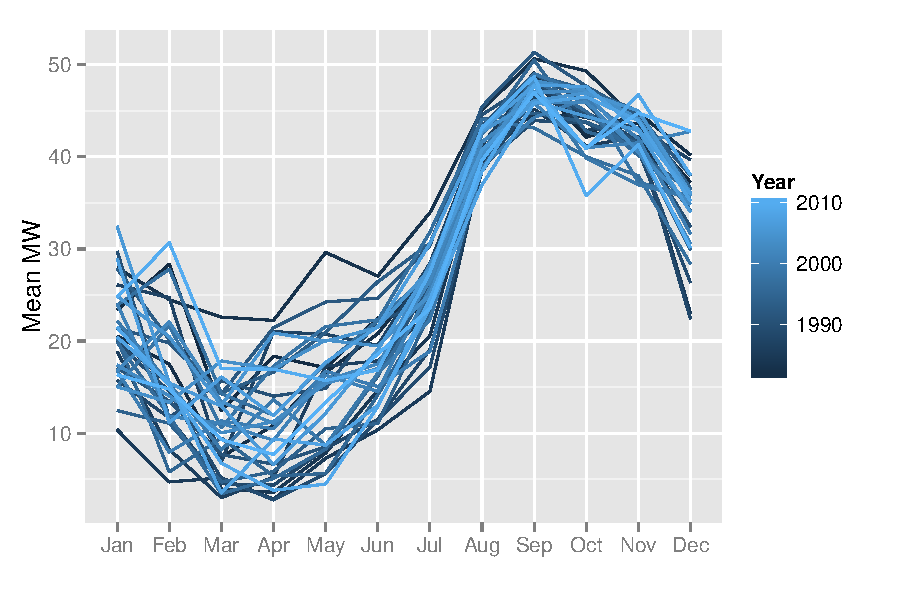
\includegraphics[width=0.8\linewidth]{./Figuras/Icaraizinho/icaraizinho-mensal}
\caption{Icaraizinho yearly data. Each serie consists of monthly observations for each year.}
\label{fig:icaraizinho-mensal}
\end{figure}


\begin{figure}
\centering
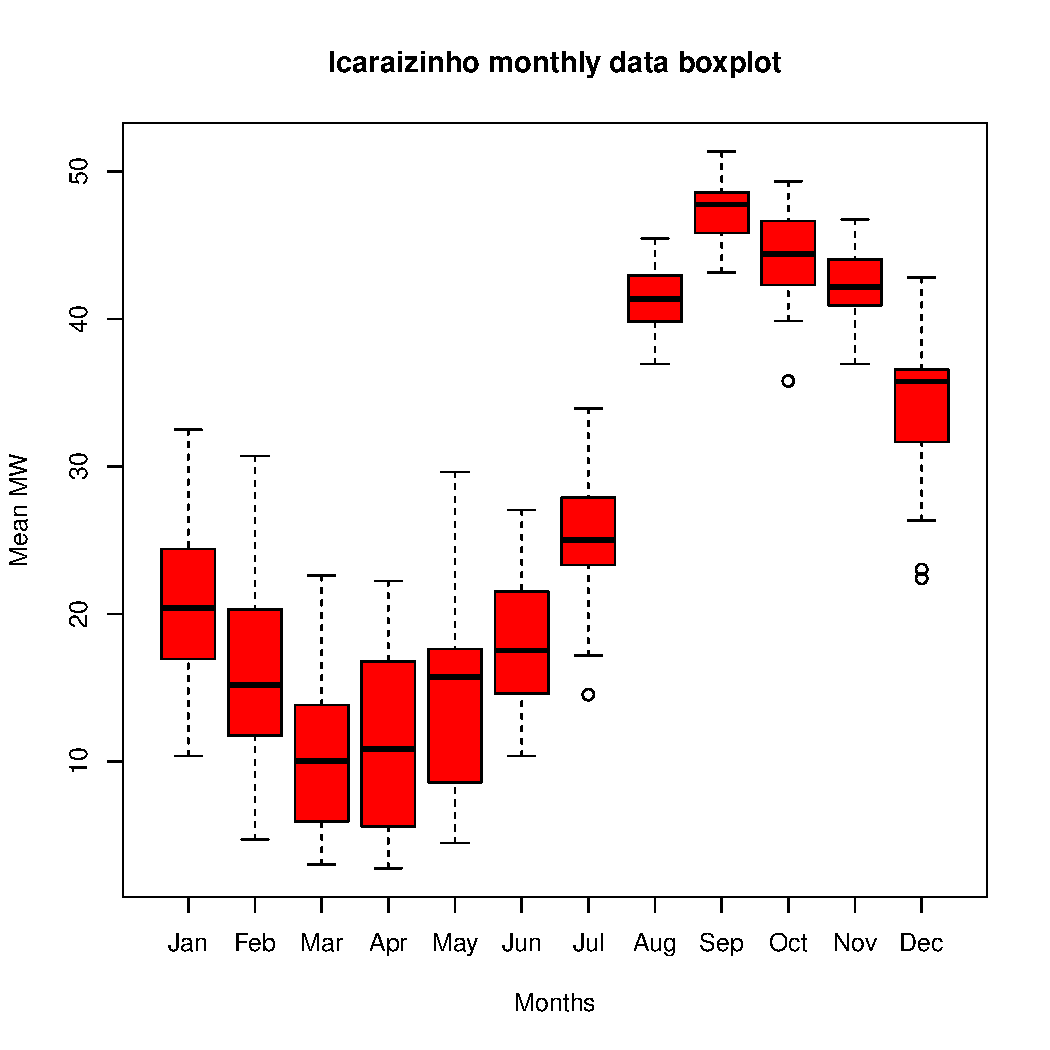
\includegraphics[width=0.8\linewidth]{./Figuras/Icaraizinho/icaraizinho-boxplot}
\caption{Boxplot for each month for the Icaraizinho dataset}
\label{fig:icaraizinho-boxplot}
\end{figure}

% % % % fadf
%\begin{figure}[htp]
%  \centering
%  \begin{minipage}[t]{0.45\linewidth}
%    \centering
%    \begin{minipage}[t]{\linewidth}
%      \centering     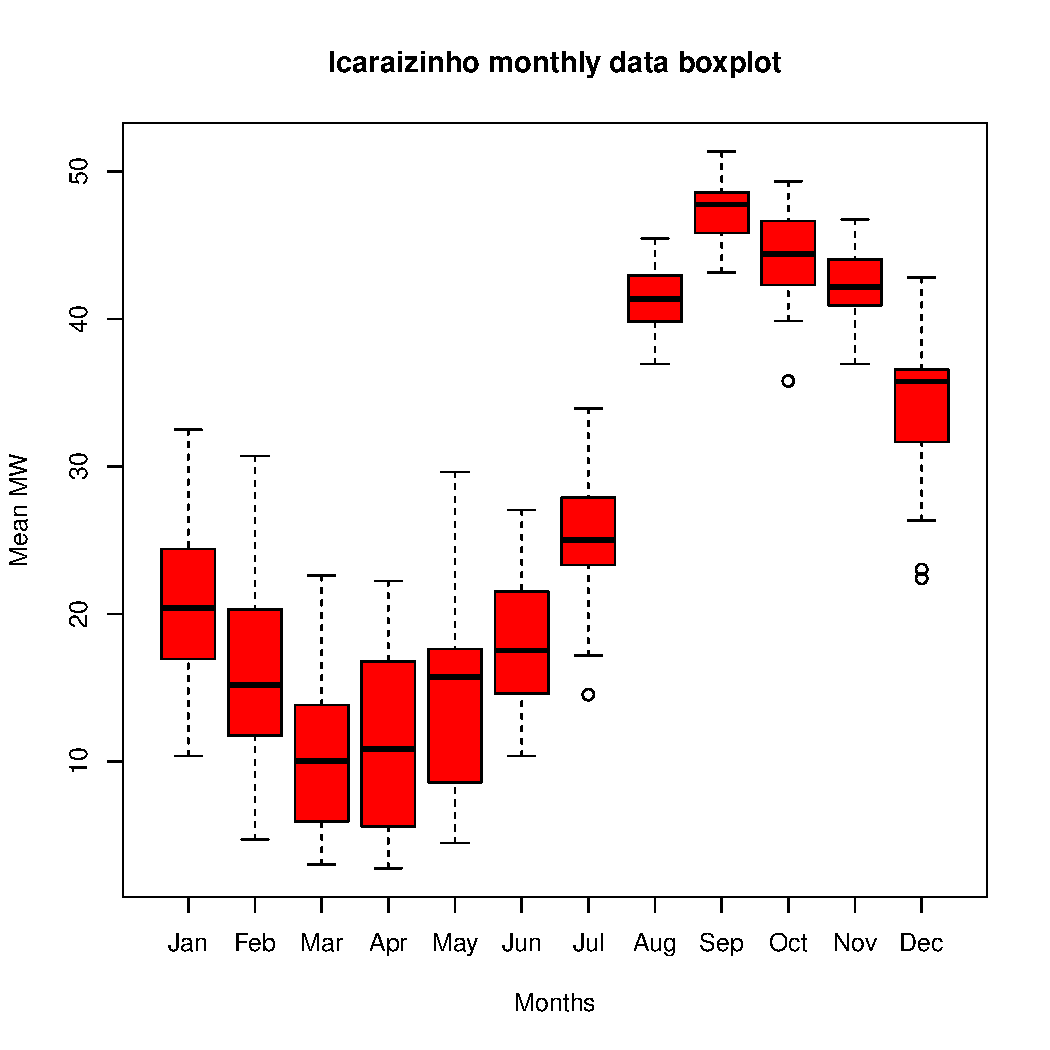
\includegraphics[width=\textwidth]{Figuras/Icaraizinho/icaraizinho-boxplot.pdf}
%      \subcaption{Monthly Boxplot}
%    \end{minipage}
%  \end{minipage}
%  \begin{minipage}[t]{0.45\linewidth}
%    \centering
%    \begin{minipage}[t]{\linewidth}
%      \centering     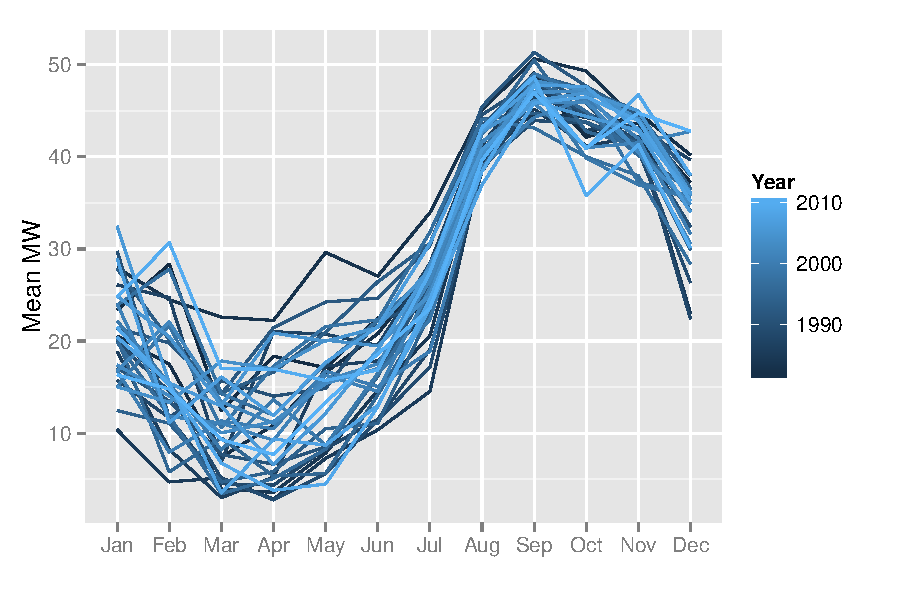
\includegraphics[width=\textwidth]{Figuras/Icaraizinho/icaraizinho-mensal.pdf}
%      \subcaption{Yearly data}
%    \end{minipage}
%  \end{minipage}
%  \caption{heading}
%  \label{fig:icaraizinho-sazonal}
%\end{figure}



\begin{figure}
  \centering
  \begin{minipage}[t]{0.45\linewidth}
    \centering
    \begin{minipage}[t]{\linewidth}
      \centering     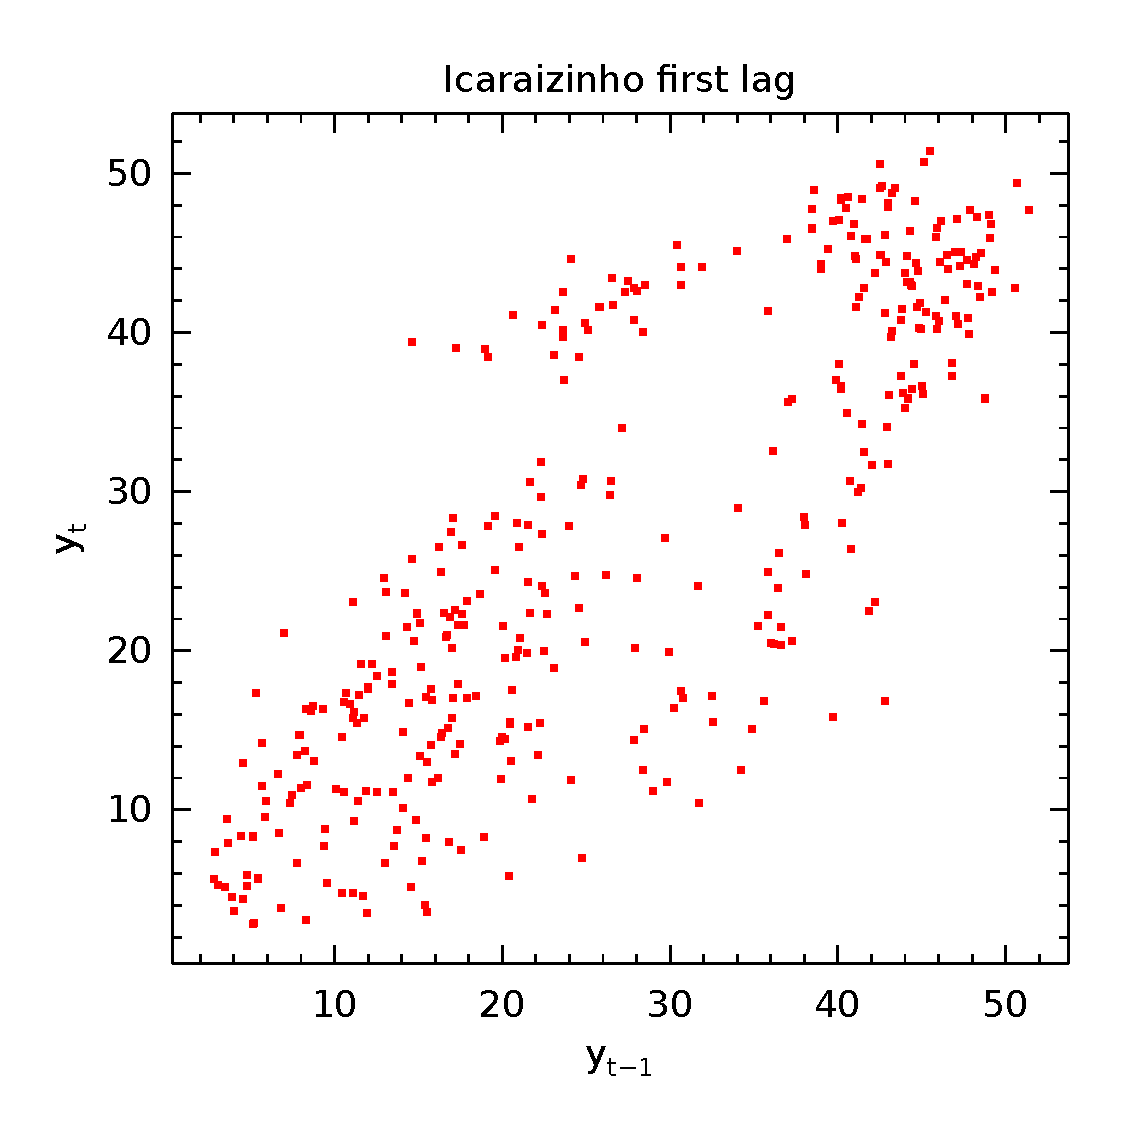
\includegraphics[width=\textwidth]{Figuras/Icaraizinho/icaraizinho-1-lag.pdf}
    \end{minipage}
    \begin{minipage}[b]{\linewidth}
      \centering     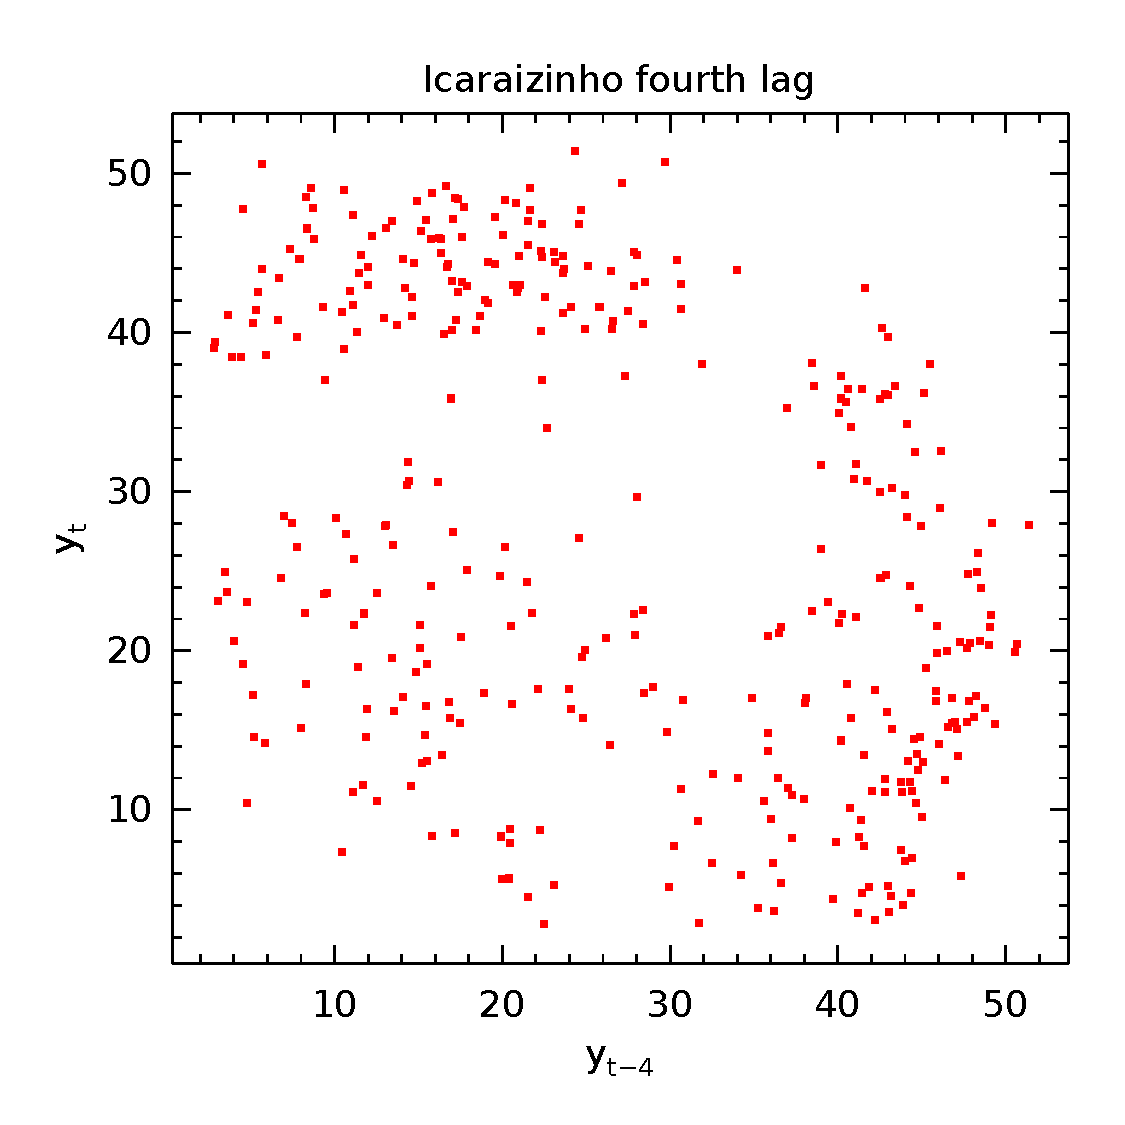
\includegraphics[width=\textwidth]{Figuras/Icaraizinho/icaraizinho-4-lag.pdf}
    \end{minipage}
  \end{minipage}
  \begin{minipage}[t]{0.45\linewidth}
    \centering
    \begin{minipage}[t]{\linewidth}
      \centering     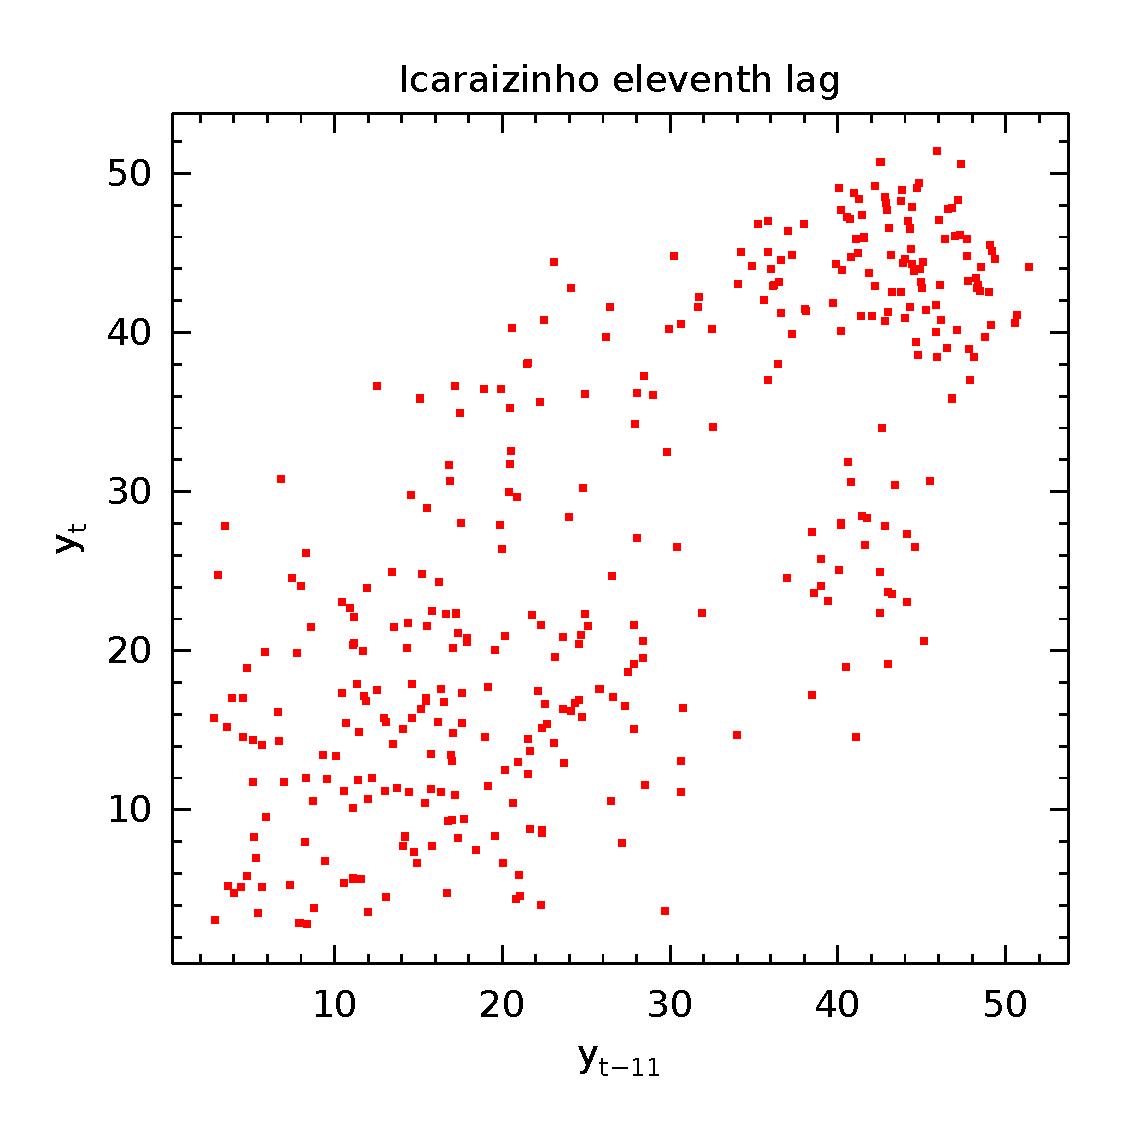
\includegraphics[width=\textwidth]{Figuras/Icaraizinho/icaraizinho-11-lag.pdf}
    \end{minipage}
    \begin{minipage}[b]{\linewidth}
      \centering     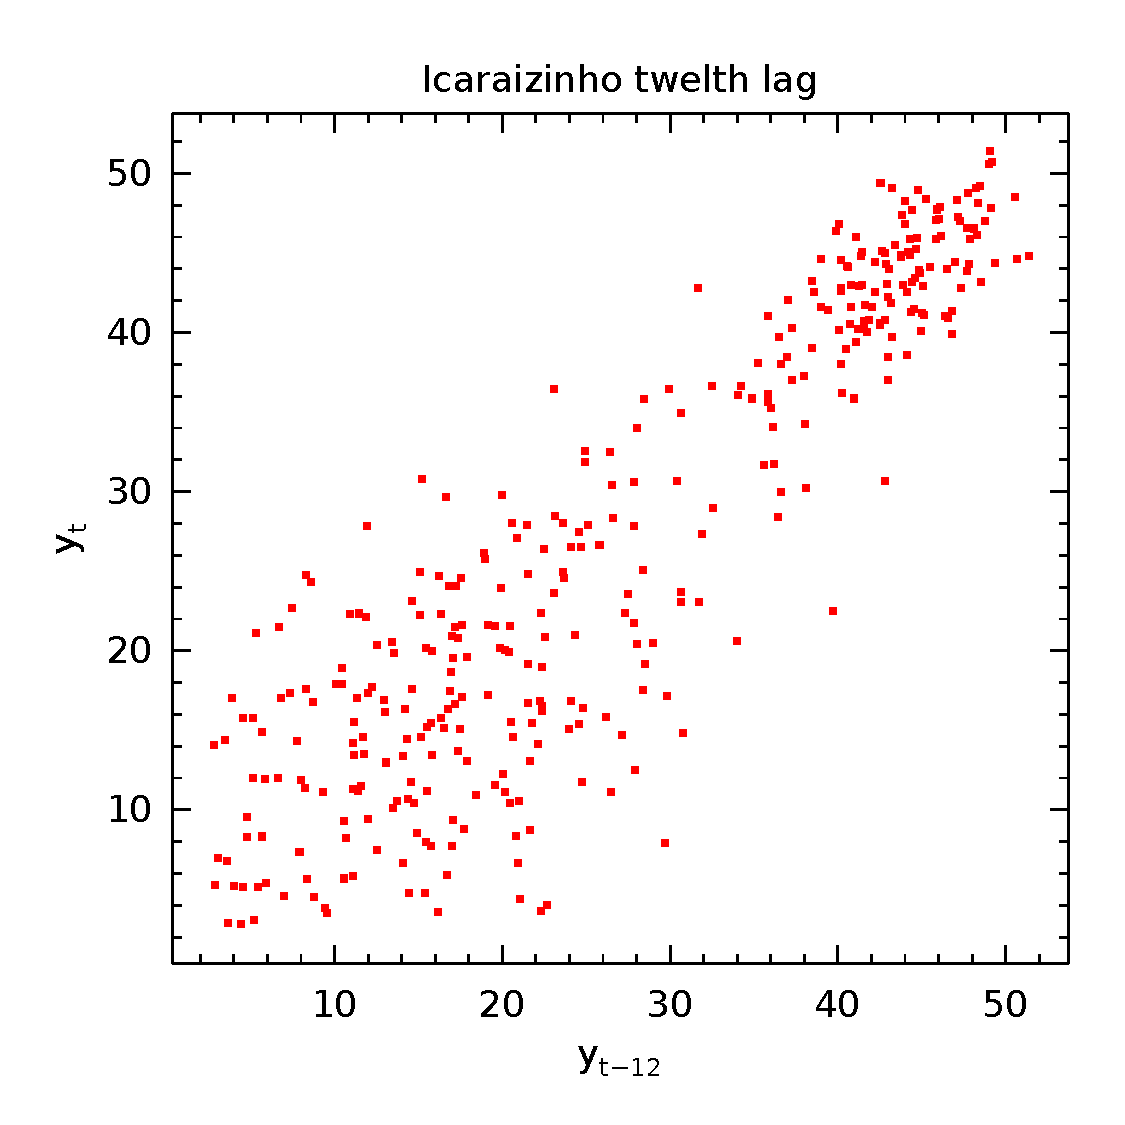
\includegraphics[width=\textwidth]{Figuras/Icaraizinho/icaraizinho-12-lag.pdf}
    \end{minipage}
  \end{minipage}
  \caption{Relationship between $y_t$ and some chosen lags.}
  \label{lags-icaraizinho}
\end{figure}

Here we denote as parametric linear model the well-known quantile regression model \cite{koenker2005quantile}. In contrast to the linear regression model through ordinary least squares (OLS), which provides only an estimation of the dependent variable conditional mean, quantile regression model yields a much more detailed information concerning the complex relationship about the dependent variable and its covariates. A Quantile Regression for the $\alpha$-quantile is the solution of the following optimization problem:
\begin{equation}
\min_{q}\sum_{t=1}^{n}\alpha|y_{t}-q(x_t)|^{+}+(1-\alpha)|y_{t}-q(x_t)|^{-},
\label{eq:linear-model}
\end{equation}
where $q(x_t)$ is the estimated quantile value at a given time $t$ and $|x|^+=\max\{0,x\}$ and $|x|^-=-\min\{0,x\}$. To model this problem as a Linear Programming problem, thus being able to use a modern solver to fit our model,  we can create variables $\varepsilon^+_t$ e $\varepsilon^-_t$ to represent $|y-q(x_t)|^+$ and $|y-q(x_t)|^-$, respectively. So we have:
\begin{equation}
\begin{aligned}\min_{q,\varepsilon_{t}^{+}, \varepsilon_{t}^{-}} & \sum_{t=1}^{n}\left(\alpha \varepsilon_{t}^{+}+(1-\alpha)\varepsilon_{t}^{-}\right) & \\
\mbox{s.t. } & \varepsilon_{t}^{+}-\varepsilon_{t}^{-}=y_{t}-q(x_{t}), & \qquad\forall t \in \{1,\dots,n\},\\
& \varepsilon_t^+,\varepsilon_t^- \geq 0, & \qquad \forall t \in \{1,\dots,n\}.
\end{aligned}
\label{eq:qar-general}
\end{equation}

Section \ref{sec:linear-models} is about linear models, so we investigate the quantile estimation when $q$ is a linear function of the series past values, up to a maximum number of lags $p$:
\begin{equation}
	q(y_t, \alpha; \beta) = \beta_0(\alpha) + \beta_1(\alpha)y_{t-1} + \beta_2(\alpha)y_{t-2} + \dots + \beta_p(\alpha) y_{t-p}.
	\label{eq:ft-qar}
\end{equation}

In section \ref{sec:npqar} we introduce a Nonparametric Quantile Autoregressive model with a $\ell_{1}$-penalty term, in order to properly simulate FEC densities for several $\alpha$-quantiles. In this nonparametric approach we don't assume any form for $q(x_t)$, but rather let the function adjust to the data. To prevent overfitting, the $\ell_1$ penalty for the second derivative (approximated by the second difference of the ordered observations) is included in the objective function.

In section 